% Chapter Template

\chapter{Methodology} % Main chapter title

\label{c4} % Change X to a consecutive number; for referencing this chapter elsewhere, use \ref{ChapterX}


\section{Data Processing}

\subsection{Enclosed Region and Target Area}
\ref{Figure 1}Latitude and longitude are geographic coordinates used to determine exact places on the Earth's surface. They are measured in degrees, with latitude representing north-south and longitude representing east-west. There are three key benefits of collecting latitude and longitude data for Indian cities as Bhuj(23.2531, 69.6693), Pokhran(27.0953, 71.7566), Jodhpur(26.2389, 73.0243), Udaipur(24.5854, 73.7175), Bengaluru(12.9716, 77.5946), Hyderabad(17.3850, 78.4867), Ahmedabad(23.0338, 72.5850), Ahmedabad2(23.0225, 72.5714), New Delhi(28.6139, 77.2090), South Delhi(28.4852, 77.1964), Ajmer(26.4499, 74.6399). The investigation focuses on a single target point many sites surrounding the target region within the limited zone. Data gathering at the specified location, a near-real-time 0.455 × 0.625-degree data set is obtained for the data from the target point. The destination location's decimal degree longitude and latitude are specified in a numeric vector format to generate this data collection. For the regional coverage, lat/log region = 381.65 meters degrees of 0.455 × 0.625 degrees. In the case study for solar irradiance forecast, a numerical vector of length eleven was used to represent the contained region. This vector contains latitude and longitude coordinates for the lower-left and upper-right corners of the enclosing box. The lower-left corner has five coordinates, and the upper-right corner has five coordinates, plus one extra value, in an 11-data vector \cite{belmahdi2020one}.

\subsection{Data Collection}
Due to a lack of ground-based temperature, it claims to have utilised historical time series and satellite data from NASA's POWER database. The data set spans 23 years, from 2001 to 2023, and consists of daily observations of solar irradiance in kilowatt-hours per square meter. This text accurately describes the data source utilised in the study; hence, it does not appear to be plagiarised. If you use this material in your work, remember to properly cite the source to give credit to the researchers who gathered and made the data available. Academic honesty and appreciating the contributions of others to research need proper citation. The forecasting challenge aims to predict solar irradiance data for a target location. Conversely, the model incorporates data from the surrounding region rather than just the target location. This strategy attempts to reduce data dependency on extraneous qualities while correcting data flaws in the target location.
High Solar Irradiance cities data was collected from eleven cities in India: Udaipur, Ajmer, Jodhpur, Pokharan, Bhuj, Hyderabad, Ahmedabad, South Delhi, New Delhi, and Bengaluru. The NASA POWER regional data access widget gave the forecasting data, which provides data access in near-real time. The objective area as well as the data region for solar irradiance. The data collecting and processing methods utilised in a case study The offered information describes methods for predicting solar irradiation. The important points are summarised here\cite{brahma2020solar}.

\begin{itemize}
\item
Deep learning models for calculating daily solar irradiation were designed and deployed as part of the research. These models were built to forecast correctly using historical data.
\item
The models were created and verified using univariate and multivariate solar irradiance data from a single location. This allowed for a comparison of the model's performance under different settings.

\item
Traditional performance evaluation measures were utilised to examine the developed models' accuracy, performance, and dependability. A rolling window assessment technique was utilised to analyse how well the models performed over time.
\item
The research examined how surrounding region characteristics affected solar irradiance forecasts for the target regions. NASA solar irradiance data gathered over 23 years was used in this investigation.

\end{itemize}

\subsection{Data Preprocessing}
Identify and manage missing values in the dataset, including imputation and row or column removal. Find and eliminate duplicate records in the dataset. Outliers are data points that differ significantly from the average and must be discovered and addressed.EDA is used to discover patterns and trends in data distribution and variable interactions. Maintain a record of all pretreatment processes and data changes. Replication requires this documentation. Examine the preprocessed data to verify if it was appropriately prepared for use as input for machine learning or deep learning models. This might include changing data or creating sequences for time series models.
\begin{itemize}
\item
Data Input: In this step, download data from NASA's website in the CSV file format; multivariate data was downloaded in Indian cities' high solar irradiant areas. The downloaded dataset is used as program input.

\item
Data Preprocessing: In this step, missing values are imputed by means. Each data work 30 iteration and 200 epochs and take the mean of all dataset.
After missing value imputing on the dataset, use min-max scaling by min-max scaling features to scale in the range [0,1].
\begin{equation}
y_{dc}=\frac{y-min(y)}{max(y)-min(y)}
\end{equation}
Here, y is the original value of a cell, min(y) is the minimum value of the column, and max(y) is the maximum value of the column.
\end{itemize}


\begin{figure}[!ht]
\centering
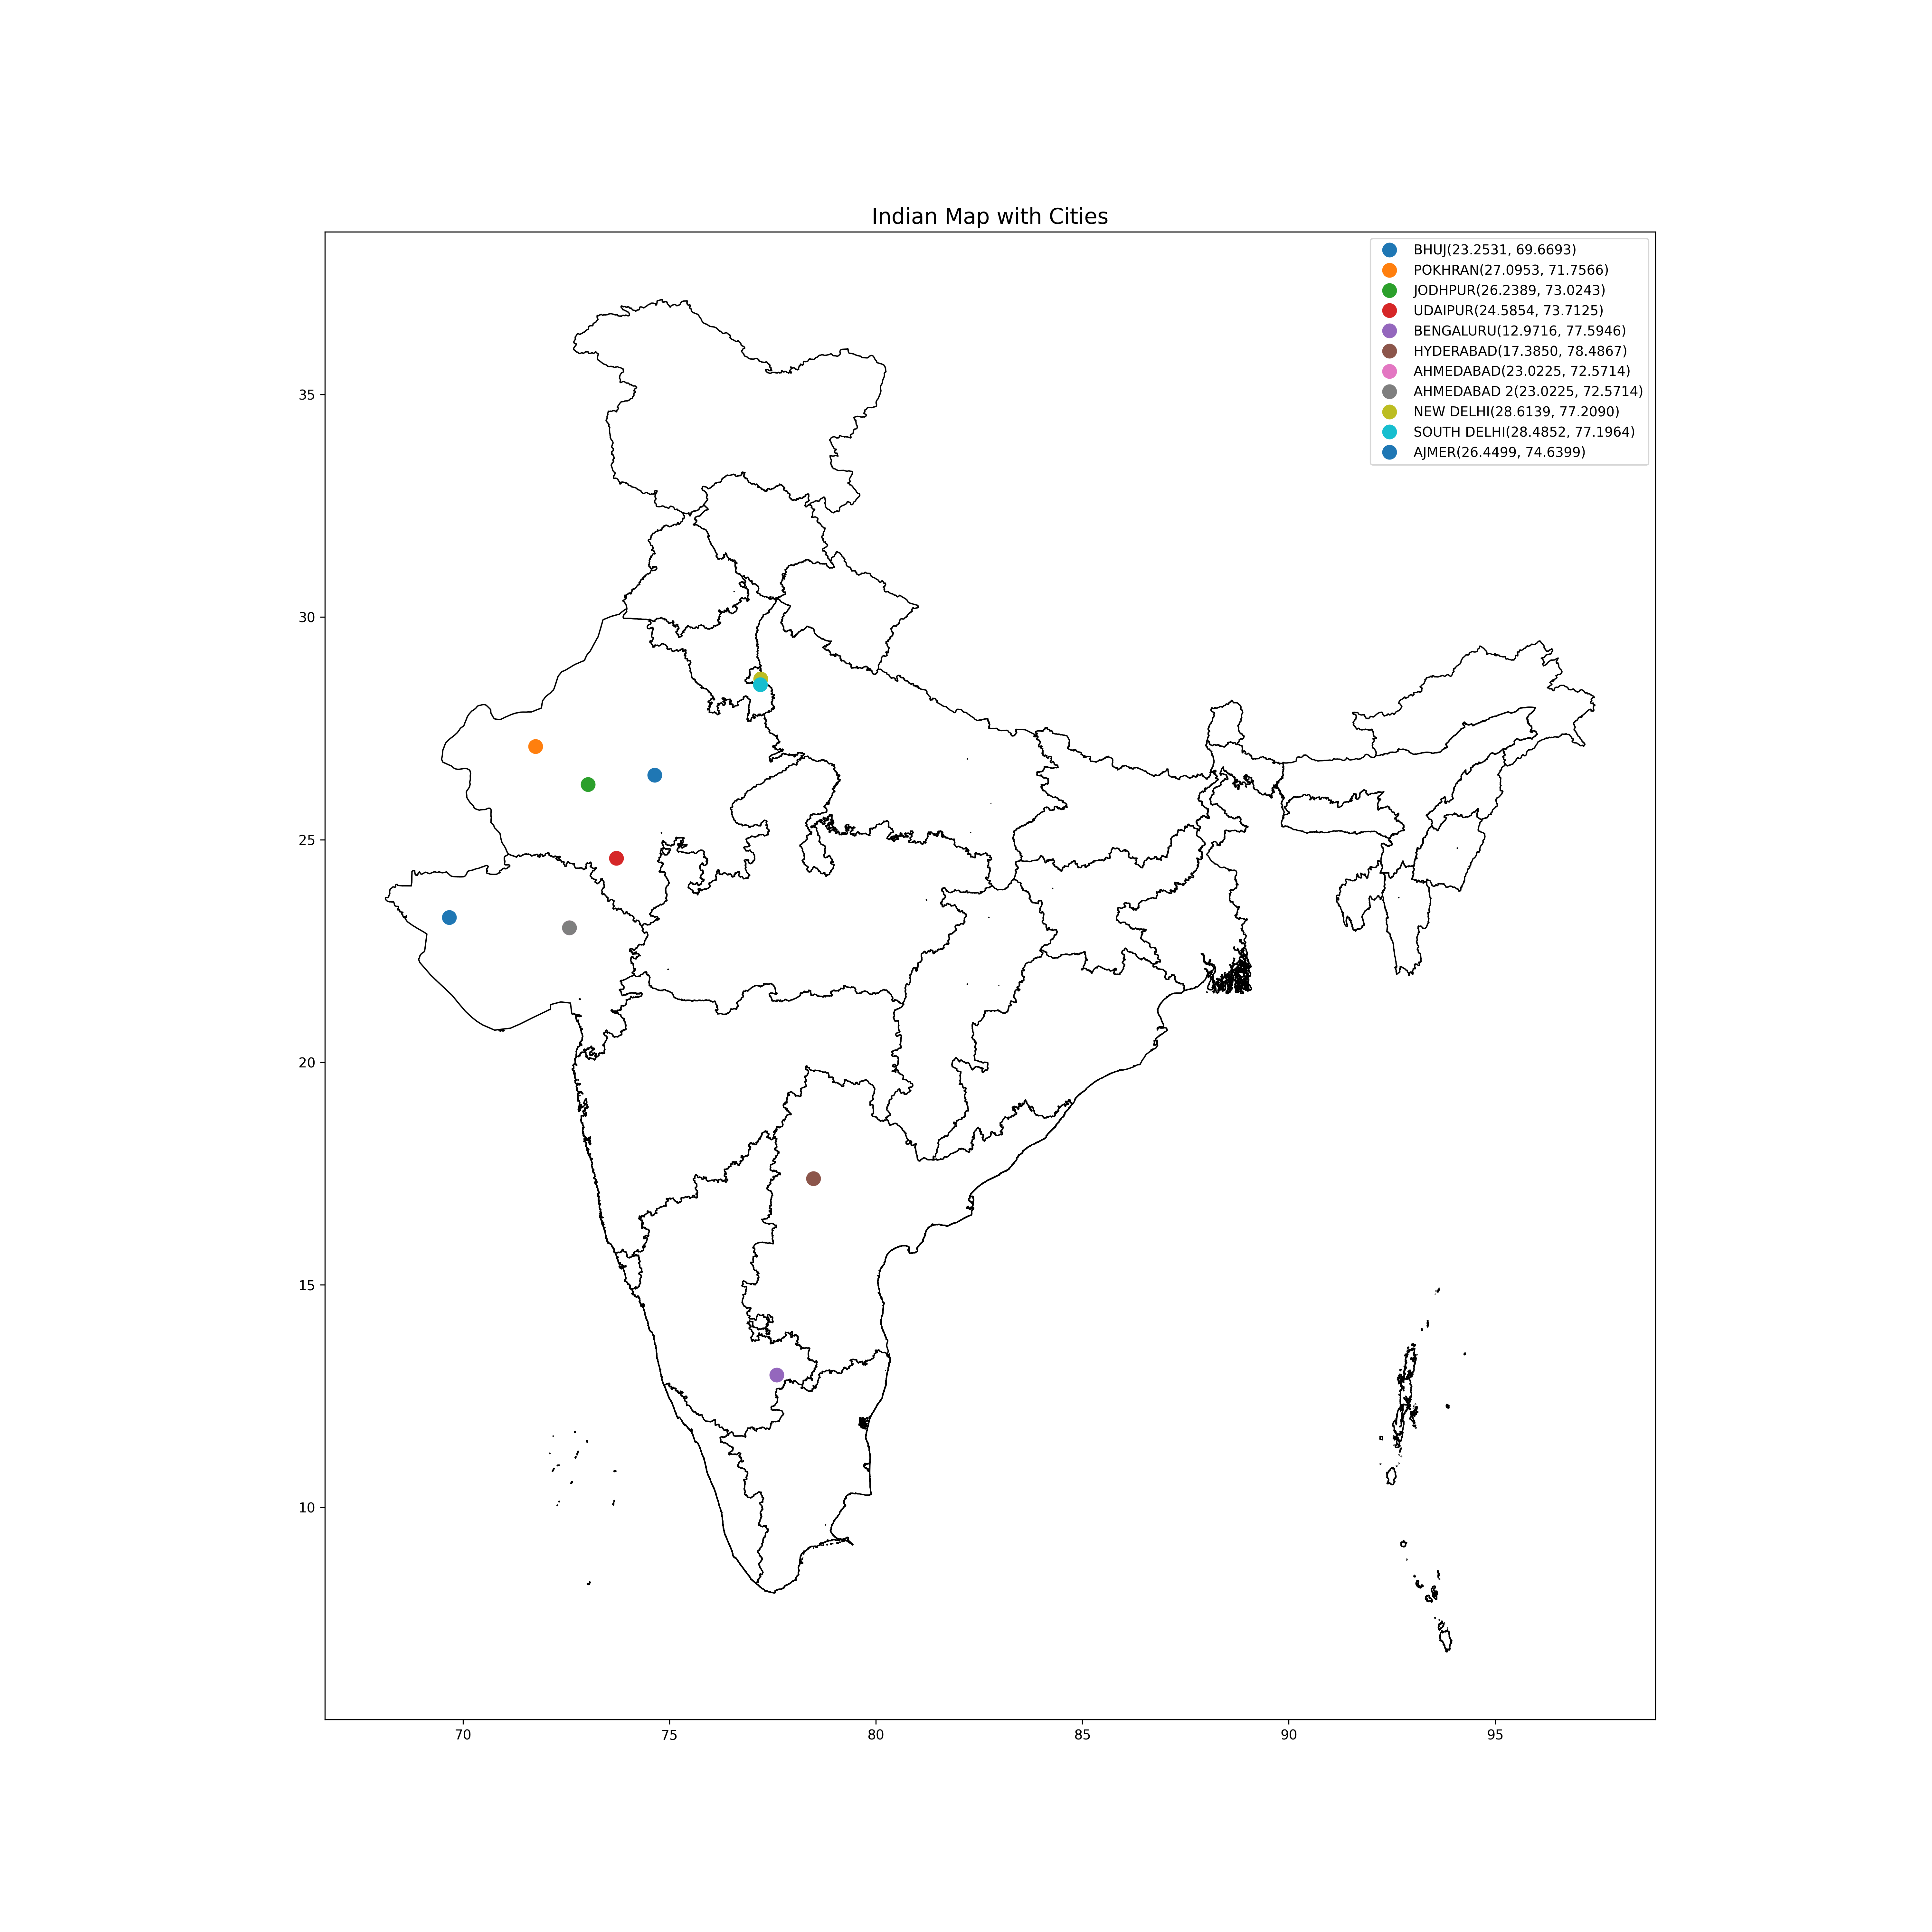
\includegraphics[width=\textwidth]{AMod India_Map}
\caption{Data location with latitude and longitude of the eleven cities of India }
\label{Figure 1}
\end{figure}

\section{Model Implementation and Evaluation}

We have proposed two hybrid models, CNN-RNN and GRU-BILSTM-LSTM, which are stand-alone where the descriptions are as follows:

\subsection{Proposed1(CNN-RNN)}A 1D Convolutional layer with 32 filters and a kernel size of 3 is added. The ReLU's activation function is employed. The input shape determines the length and number of features in the sequences. A MaxPooling layer with a pool size of 2 is added. As a result, the dimensionality of the feature maps is decreased. Another Conv1D layer is added this time with 64 filters and kernel size 3. ReLU activation is used.
Another MaxPooling layer with pool size two is added.\\
\textbf{Model Compilation:} The model is built using the Adam optimiser and the MAE loss function. The model summary function generates a summary of the model's architecture, including the layer types, output shapes, and total number of parameters shown in Figure 2. This architecture combines the capabilities of CNNs (for feature extraction) with RNNs (for sequence modelling) to address applications that need sequential data. The CNN layers are responsible for learning hierarchical features, whereas the LSTM layer is responsible for acquiring sequential patterns. The model's performance is affected by the subject and dataset to which it is applied. More fine-tuning and testing may be necessary for the best results.




\begin{figure}[!ht]
\centering
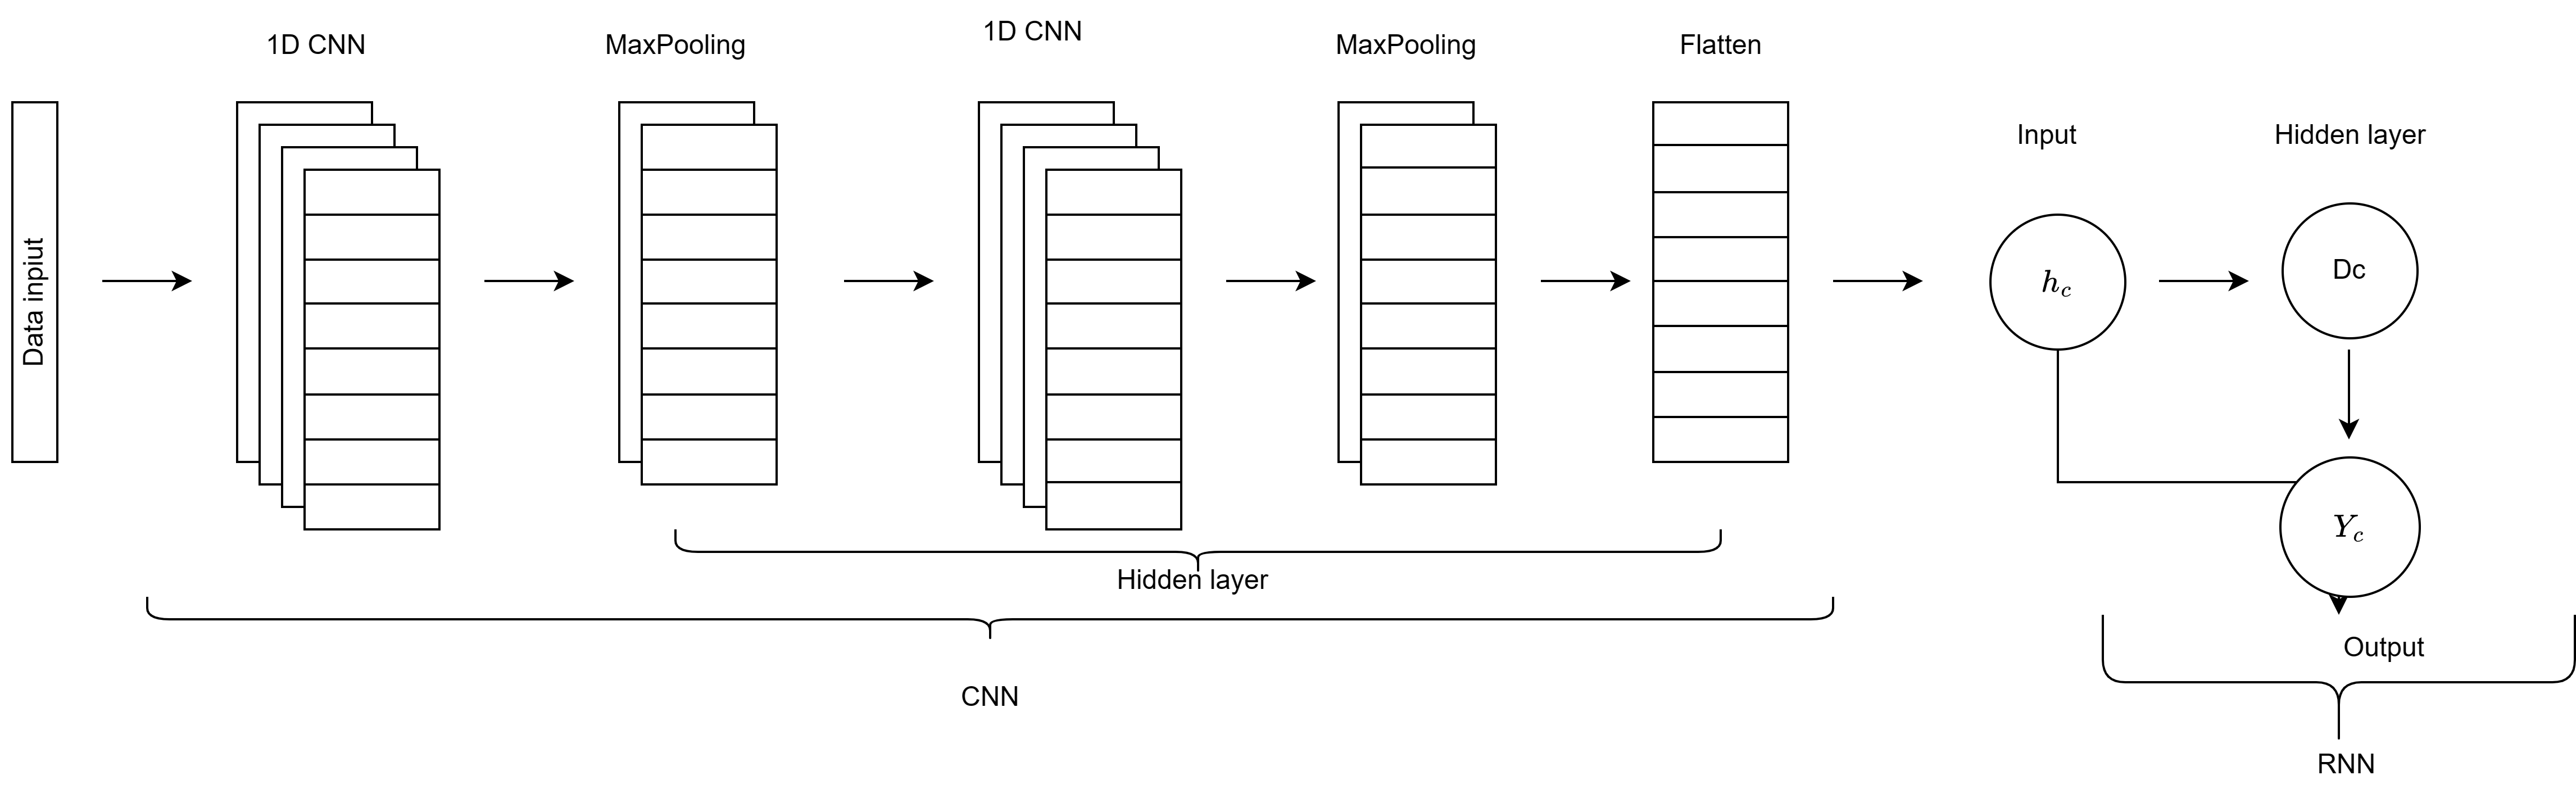
\includegraphics[width=\textwidth]{CNN-RNN (1)}
\caption{Architecture of Proposed1(CNN-RNN)}
\label{}
\end{figure}





1. Convolutional Layer:
\begin{equation}
\mathbf{Z}_{\text{conv}} = \mathbf{D}_{\text{conv}} * \mathbf{X} + \mathbf{b}_{\text{conv}}
\end{equation}

2. Activation Function for Convolutional Layer:
\begin{equation}
\mathbf{A}_{\text{conv}} = \sigma(\mathbf{Z}_{\text{conv}})
\end{equation}

3. Reshape for RNN Input:
\begin{equation}
\mathbf{X}_{\text{rnn}} = \text{reshape}(\mathbf{A}_{\text{conv}})
\end{equation}

4. RNN Hidden State Update:
\begin{equation}
\mathbf{h}_c = \tanh(\mathbf{D}_{\text{rnn}} \cdot \mathbf{h}_{c-1} + \mathbf{D}_{\text{xrnn}} \cdot \mathbf{x}_c + \mathbf{b}_{\text{rnn}})
\end{equation}

5. RNN Output Calculation:
\begin{equation}
\mathbf{Y}_c = \mathbf{D}_{\text{out}} \cdot \mathbf{h}_c + \mathbf{b}_{\text{out}}
\end{equation}

In this case, the convolutional filter weights are represented by $\mathbf{D}_\text{conv}$. The input data is represented by $\mathbf{X}$. The bias term for the convolutional layer is $\mathbf{b}_\text{conv}$, while the activation function (e.g., ReLU) for the convolutional layer is $sigma$. The activation map from the convolutional layer is $\mathbf{A}_\text{conv}$. $\text{reshape}$ is used to reshape the activation map for RNN input. The weight matrix for the RNN hidden state update is $\mathbf{D}_\text{rnn}$, the weight matrix for the RNN input is $\mathbf{b}_\text{rnn}$, and the bias term for the RNN is $\mathbf{b}_\text{rnn}$. $\mathbf{h}_c$ represents the RNN hidden state at time step $c$, $\mathbf{x}_c$ represents the input at time step $c$, $\mathbf{D}_\text{out}$ represents the weight matrix for the RNN output computation, $\mathbf{b}_\text{out}$ represents the bias term for the RNN output, and $\mathbf{Y}_c$ represents the output at time step $c$.



\subsection{Proposed2(GRU-BILSTM-LSTM)}
\textbf{layer1:}A GRU layer with the requisite number of units is added. It is set to return sequences (return-sequences=True) and requires shape data as input.
A BiLSTM layer is used. This layer explores sequences both forward and backwards, providing more background information.\\
\textbf{layer2:} An extra LSTM layer is added. It, like the first GRU layer, returns sequences. A dropout layer is used to prevent overfitting. It encourages regularisation by randomly changing during training; some input units are set to zero updates. Another GRU layer is added that does not return sequences.
Another dropout layer follows the second GRU layer. A connected thick layer of 1 unit is applied to the final product. It gives back a single scalar forecast.

\textbf{Model Compilation:}The Adam optimiser, an adaptive learning rate optimisation technique, is used to build the model. The loss function used is MAE, which determines the absolute difference between expected and actual data. To conclude, this model employs regularisation dropout and recurrent layers GRU, Bidirectional LSTM, and LSTM. The objective is to create a complex architecture that recognises temporal patterns in sequential data. The MAE loss is used for training, and the model is designed to generate a single prediction for the given input sequence.



\begin{figure}[!ht]
\centering
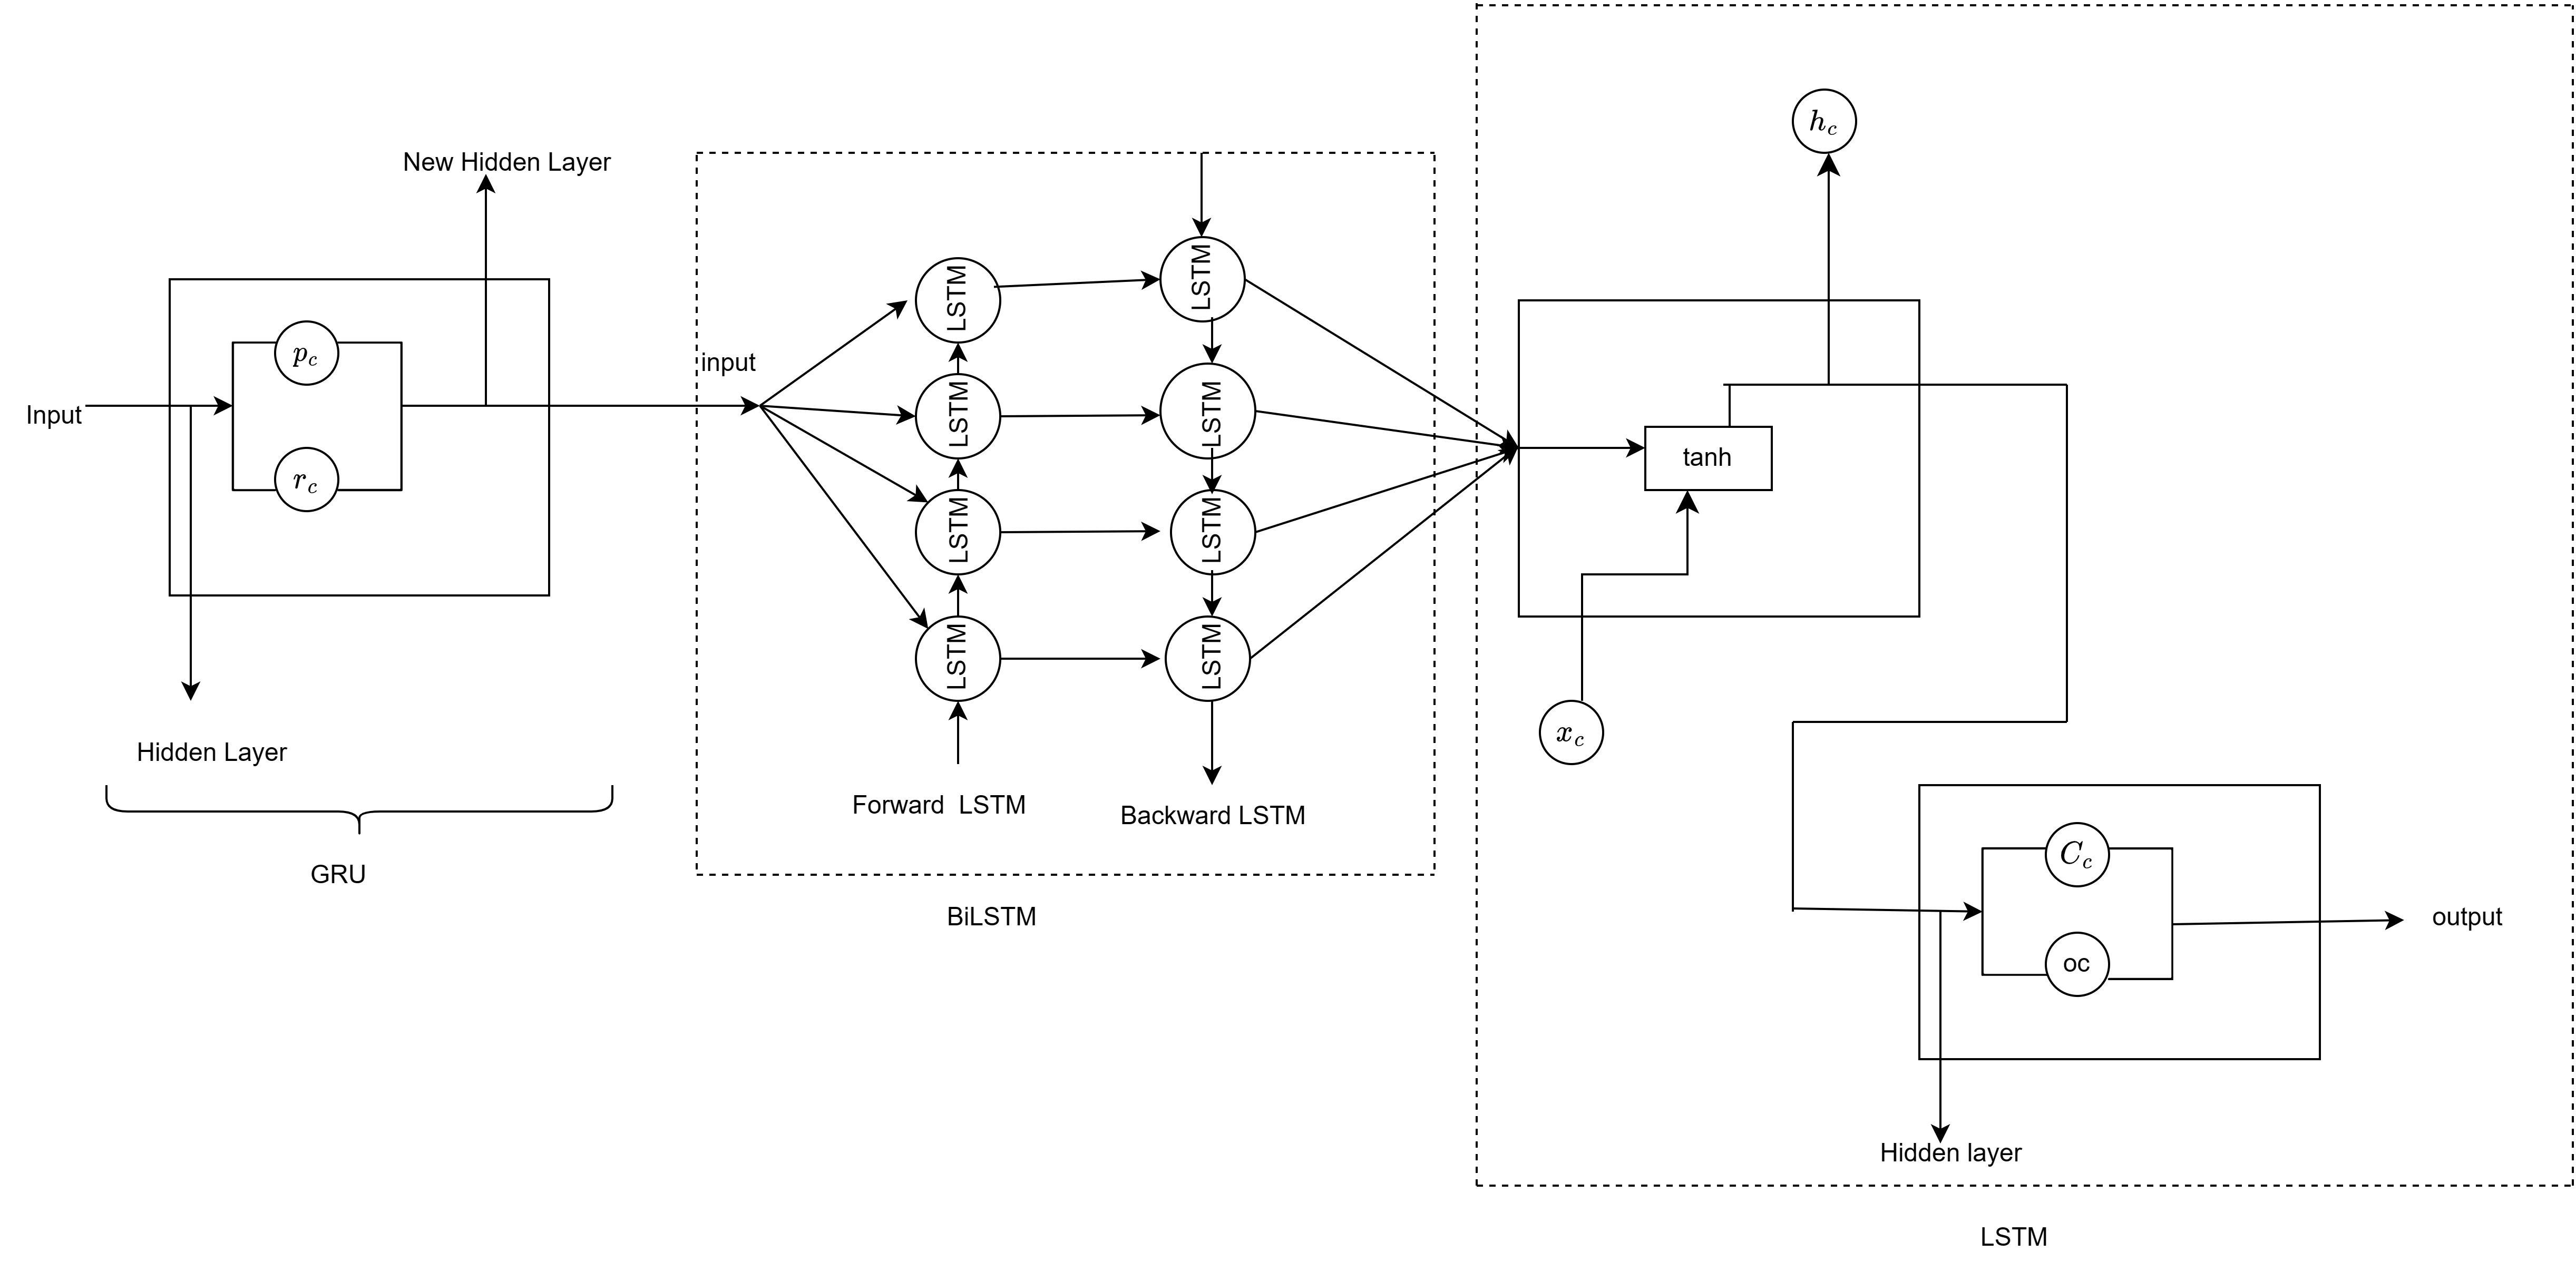
\includegraphics[width=\textwidth]{GRU-BiLSTM-LSTM (1)}
\caption{Architecture of Proposed2(GRU-BiLSTM-LSTM)}
\label{}
\end{figure}




1. GRU Equations:
(Update Gate$z_c$):
\begin{equation}
p_c = \sigma(D_z \cdot [h_{c-1}, x_c])
\end{equation}

Reset Gate ($r_c$):
\begin{equation}
r_c = \sigma(D_r \cdot [h_{c-1}, x_c])
\end{equation}

Candidate Memory ($\tilde{h}_c$):
\begin{equation}
\tilde{h}_c = \tanh(D_h \cdot [r_c \odot h_{c-1}, x_c])
\end{equation}

Hidden State Update ($h_c$):
\begin{equation}
h_c = (1 - z_c) \odot h_{c-1} + z_c \odot \tilde{h}_c
\end{equation}

2. Bidirectional LSTM Equations:
Forward(F) LSTM:
(Similar to LSTM equations)

Backward(B) LSTM:
(Similar to LSTM equations)

3. LSTM Equations:
Forget Gate:
\begin{equation}
f_c = \sigma(D_f \cdot [h_{c-1}, x_c] + b_f)
\end{equation}

Input Gate:
\begin{equation}
i_c = \sigma(D_i \cdot [h_{c-1}, x_c] + b_i)
\end{equation}

Candidate Memory:
\begin{equation}
\tilde{C}_c = \tanh(D_C \cdot [h_{c-1}, x_c] + b_C)
\end{equation}

Update Memory:
\begin{equation}
C_c = f_c \odot C_{c-1} + i_c \odot \tilde{C}_c
\end{equation}

Output Gate:
\begin{equation}
o_c = \sigma(D_o \cdot [h_{c-1}, x_c] + b_o)
\end{equation}

Hidden State:
\begin{equation}
h_c = o_c \odot \tanh(C_c)
\end{equation}

The sigmoid activation function is represented by $\sigma$, the hyperbolic tangent activation function is represented by $tanh$, the weight matrices and bias terms are represented by $D$ and $b$, the input at time step $c$ is represented by $x_c$, and the prior hidden state is represented by $h_{c-1}$, $z_c$, $r_c$, $\tilde{h}_c$, $h_c$ are the GRU update gate, reset gate, candidate memory, and hidden state respectively. The Bidirectional LSTM equations are similar to regular LSTM equations, and the LSTM equations are standard. The model combines these three recurrent layer types to process sequential data.



\begin{table}[!ht]
  \centering
  \setlength{\tabcolsep}{3pt}
  {\renewcommand{\arraystretch}{1}%
  \caption{Values of Parameter of Models}
  %\label{Algorithm Parameters-table}
  \begin{tabular}{|p{0.4 \textwidth}| p{0.4 \textwidth}|}
  \hline
  Algorithm Parameters & Values \\ \hline
  filter & 32 \\
  kernel sise & 3 \\
  MaxPooling & 2 \\
  Activation & ReLU \\
  Optimizer & Adam \\
  Loss Function & MSE \\ \hline
  \label{Table 2}
  \end{tabular}%
  }
  \end{table}
  
  
  \subsection{Experimental Setup} The most critical algorithm parameters and their values are shown in the table below. The "Filter Count" option is set to 32, indicating the number of filters or convolutional units used in a convolutional layer. The option "Kernel Size" is set to 3, indicating that the convolutional kernel used in feature extraction has a size of 3. The "MaxPooling" option is set to 2, indicating that a MaxPooling operation with a pool size 2x2 is being used. The "ReLU" (Rectified Linear Unit) function is utilised for the activation function, a common choice in neural networks to generate non-linearity. The "Adam" optimiser is used during training to update the network's weights, and the "Mean Squared Error" (MSE) is utilised as the loss function to compare the model's prediction accuracy against actual values shown in Table \ref{Table 2}.
  